\documentclass{beamer}
\usepackage{../tut-slides}
\usepackage{../mathoperatorsAuD}

\usepackage{csquotes}
\usepackage{cancel}

\usepackage{amsmath,amssymb}

\usepackage{tikz}
\usetikzlibrary{positioning,automata, matrix, trees}
\usetikzlibrary{calc,positioning,backgrounds,arrows.meta}
\usetikzlibrary{patterns,snakes}
\usepackage{forest}


\usepackage{booktabs}
\usepackage{tabularx}
\usepackage{tabu}
\newcommand*\head{\rowfont{\bfseries}}
\newcommand*{\tw}{\rowfont{\ttfamily}}

\renewcommand{\tabularxcolumn}[1]{>{\hspace{0pt}}m{#1}}

\usepackage{listings}
\usepackage{textgreek}


\renewcommand{\emph}[1]{\textbf{#1}}
\newcommand{\coloremph}[1]{\textcolor{cdpurple}{#1}}
\newcommand{\col}[1]{\textcolor{cdpurple}{\boldsymbol{#1}}}
\newcommand{\coll}[1]{\textcolor{cddarkgreen}{\boldsymbol{#1}}}
\newcommand{\colll}[1]{\textcolor{cdorange}{\boldsymbol{#1}}}
%\newcommand{\step}[2][]{\ensuremath{\overset{{#1} (\text{#2})}{=}}}
%\newcommand*{\astep}[2][]{\ensuremath{\overset{{#1} (\text{#2})}&{=}}}

\newcommand{\num}[1]{\ensuremath{\langle #1 \rangle}}

\undef\trans
\DeclareMathOperator{\trans}{trans}

\newcommand{\logand}{ \ \land \ }

\begin{document}	
	\title{Programmierung}
	\subtitle{Übung 12: Hoare-Kalkül}
	\author{Eric Kunze}
	\email{eric.kunze@tu-dresden.de}
	\city{TU Dresden}
	\date{06. Juli 2022}
%	\institute{Lehrstuhl für Grundlagen der Programmierung}
	\titlegraphic{
\includegraphics[width=2cm]{../TUD-white.pdf}}
	
	\maketitle
	

%%%%%%%%%%%%%%%%%%%%%%%%%%%%%%%%%%%%%%%%%%%%%%%%%%%%%%%%%%%%%%%%%%%%%%%%%%%%%

\begin{frame}[fragile] \frametitle{Inhalt}
	\begin{enumerate}
		\item Funktionale Programmierung
		\begin{enumerate}
			\item Einführung in Haskell: Listen
			\item Algebraische Datentypen
			\item Funktionen höherer Ordnung
			\item Typpolymorphie \& Unifikation
			\item Beweis von Programmeigenschaften
			\item \textlambda--Kalkül
		\end{enumerate}
		\item Logikprogrammierung
		\item Implementierung einer imperativen Programmiersprache
		\begin{enumerate}
			\item Implementierung von C${}_\text{0}$
			\item Implementierung von C${}_\text{1}$
		\end{enumerate}
		\item \textbf{Verifikation von Programmeigenschaften}
		\item H${}_\text{0}$ -- ein einfacher Kern von Haskell
	\end{enumerate}
\end{frame}



\section{\textsc{Hoare}-Kalkül}

\begin{frame} \frametitle{\textsc{Hoare}-Kalkül}
	\begin{itemize}
		\item Beweis / Verifikation von Programmeigenschaften \pause 
		\item Verifikationsformeln der Form $\{P\} \ \mathbf{A} \ \{Q\}$
		\begin{itemize}
			\item $P$ und $Q$ sind Zusicherungen (prädikatenlogische Ausdrücke)
			\item $P$ heißt \emph{Vorbedingung}, $Q$ heißt \emph{Nachbedingung}
			\item Beschreibung der Veränderung von Zusicherungen \pause
			\item \emph{Bedeutung}: Wenn die Variablenwerte vor Ausführung von $\mathbf{A}$ die Zusicherung $P$ erfüllen und $\mathbf{A}$ terminiert, dann erfüllen die Variablen nach Ausführung von $\mathbf{A}$ die Zusicherung $Q$
		\end{itemize} \pause
		\item Aufstellen eines Beweisbaumes mit zur Verfügung stehenden Regeln
	\end{itemize}
\end{frame}


\begin{frame} \frametitle{\textsc{Hoare}-Kalkül --- Regeln}
	\begin{itemize}
		\item Zuweisungsaxiom
		\item Sequenzregel
		\item CompRegel
		\item Iterationsregel
		\item (erste und zweite) Alternativregel
		\item Konsequenzregeln
		\begin{itemize}
			\item stärkere Vorbedingung
			\item schwächere Nachbedingung
		\end{itemize}
	\end{itemize}
\end{frame}

\begin{frame} \frametitle{Schleifeninvariante}
	Für die Iterationsregel benötigen wir die Schleifeninvariante $SI$.
	In den meisten unserer Fälle ist diese von der Form $SI = A \land B$, wobei
	\begin{itemize}
		\item $A$ den Zusammenhang zwischen Zählvariable und Akkumulationsvariablen beschreibt. Führe dazu einige Iterationen der Schleife durch und leite daraus einen Zusammenhang her.
		\item $B$ die abgeschwächte Schleifenbedingung ist. Dabei nehmen wir die letztmögliche Variablenbelegung, für die die Schleifenbedingung $\pi$ noch wahr ist und führen den Schleifenrumpf noch einmal darauf aus ($\to \pi'$). \\
		$\leadsto B = \pi \cup \pi'$
	\end{itemize}
\end{frame}



\section{Aufgabe 1}

\begin{frame}[t] \frametitle{Aufgabe 1 -- Teil (a)}
	\footnotesize
	\textbf{Verfikationsformel:}
	\begin{scriptsize}
		\setlength\arraycolsep{1pt}
		\begin{equation*}
			\underbrace{ \left\{ \begin{array}{cccc}
					      & (k \ge 0) &\land& (u \ge k) \\
					\land & (j = k)   &\land& (s = 0)
				\end{array}
			\right\}}_{\text{Vorbedingung}} \ \ \texttt{\emph{while} (\texttt{j} < \texttt{u}) \{ \texttt{j=j+1; s=j+s;}; \}} \ \ \underbrace{ \left\{
				s = \frac{\texttt{u}^2 + \texttt{u} - \texttt{k}^2 - \texttt{k}}{2}
			\right\}}_{\text{Nachbedingung}}
		\end{equation*}
	\end{scriptsize}
	
	
	\pause
	
	\textbf{Schleifeninvariante:} $\qquad$ $SI = A \land B$ \pause
	
	\begin{minipage}{\dimexpr0.6\linewidth-\fboxrule-\fboxsep}
		\begin{center}
			\begin{tabular}{|c||l|r|}
				\hline
				$\#$ & \texttt{j} & \texttt{s} \\
				\hline\hline
				$0$	 & $k$   & $0$  \\
				$1$  & $k+1$ & $(k+1)$  \\
				$2$  & $k+2$ & $(k+2) + (k+1)$ \\
				$\vdots$ & $\vdots$ & $\vdots$ \\
				$N$  & $k+N$ & $(k+N) + \dots + (k+1)$ \\
				\hline
			\end{tabular}
		\end{center}
	\end{minipage}
	\begin{minipage}{\dimexpr0.4\linewidth-\fboxrule-\fboxsep}
		\centering
		Als Gleichungssystem:
		\begin{equation*}
			\begin{array}{rl}
			\texttt{j} &= k + N \\ \texttt{s} &= \sum\limits_{i = k+1}^{k+N} i
			\end{array}
		\end{equation*}
		$\Rightarrow \enskip A = (s = \sum\limits_{i = k+1}^j i)$		
	\end{minipage}
\end{frame}

\begin{frame}[t] \frametitle{Aufgabe 1 -- Teil (a)}
	\fbox{$SI = A \land B$} und wir wissen schon $A = (s = \sum\limits_{i = k+1}^j i)$
	
	\bigskip
	
	\textbf{abgeschwächte Schleifenbedingung:}
	\begin{itemize}
		\item Schleifenbedingung: \onslide<2->{$\pi = (\texttt{j < u})$}
		\item Schleifenbedingung letztmalig wahr für \onslide<2->{\texttt{j = u - 1}}
		\item Wert nach nochmaligem Schleifendurchlauf: \onslide<2->{$\pi' = (\texttt{j = u})$}
		\item $B = \pi \cup \pi' = \onslide<2->{(\texttt{j} \le \texttt{u})}$ \hspace{1cm} {\footnotesize \itshape (symbolische Schreibweise)}
	\end{itemize}
	\medskip
	\pause
	\fbox{$\Longrightarrow SI = A \land B = (s = \sum\limits_{i = k+1}^j i) \land (\texttt{j} \le \texttt{u})$}
\end{frame}

\begin{frame}[t] \frametitle{Aufgabe 1 -- Teil (b)}
	\small	
	Sei $SI = A \land B = \left( s = \sum\limits_{i = k+1}^j i \right) \land (j \le u)$ und $\pi = (j < u)$.
	
	\begin{center}
		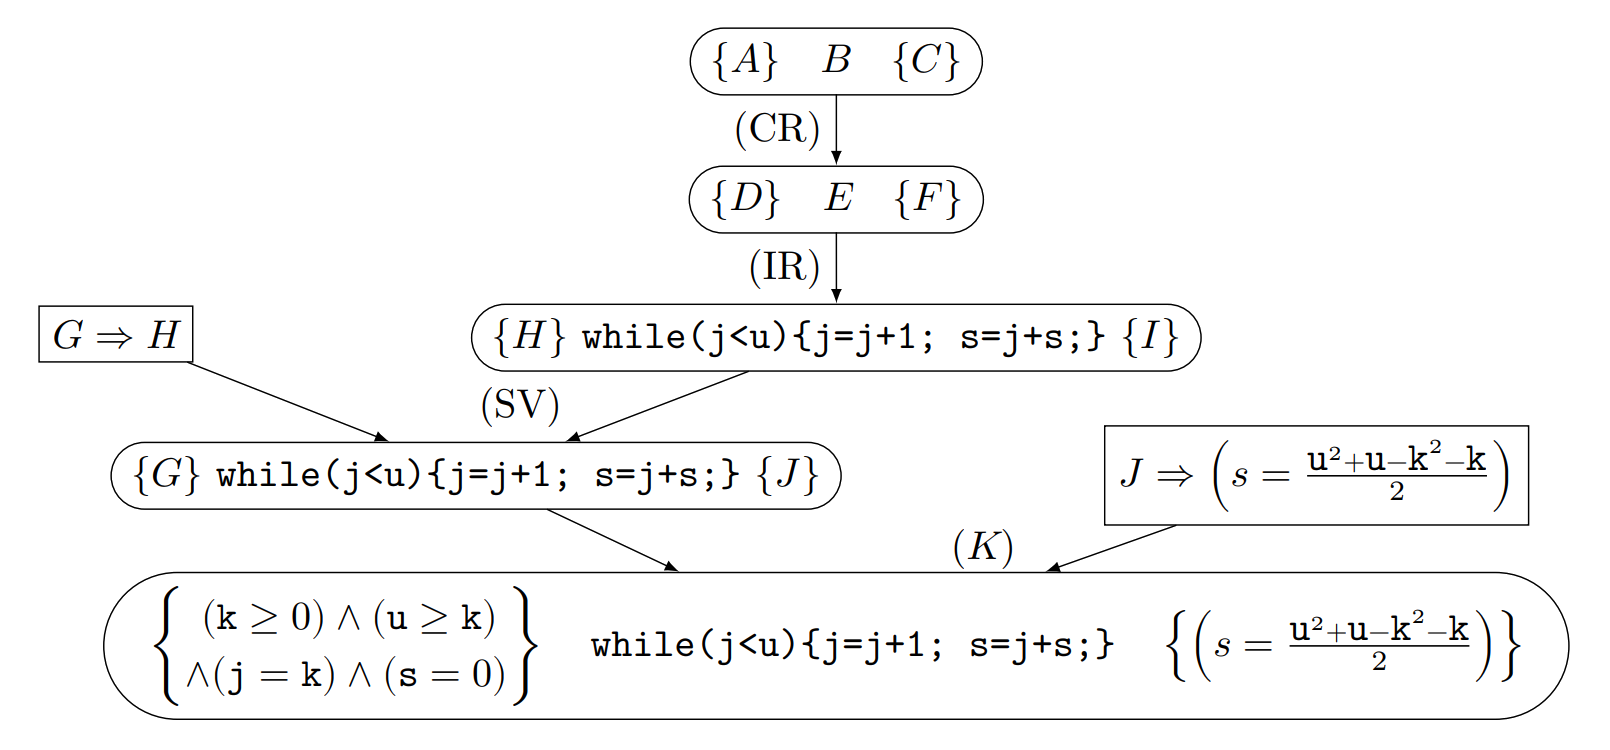
\includegraphics[width=\linewidth]{tut12-aufgabe1-baum.png}
	\end{center}
\end{frame}

\begin{frame} \frametitle{Aufgabe 1 -- Teil (b)}
	\small
	
	\begin{center}
		\emph{Verfikationsformel:} 
		\begin{scriptsize}
			\setlength\arraycolsep{1pt}
			\begin{equation*}
				\left\{ \begin{array}{cccc}
						& (k \ge 0) &\land& (u \ge k) \\
						\land & (j = k)   &\land& (s = 0)
					\end{array}
					\right\} \ \ \texttt{\emph{while} (\texttt{j} < \texttt{u}) \{ \texttt{j=j+1; s=j+s;}; \}} \ \ \left\{
					s = \frac{\texttt{u}^2 + \texttt{u} - \texttt{k}^2 - \texttt{k}}{2}
					\right\}
			\end{equation*}
		\end{scriptsize}
	\end{center}
	
	\bigskip
	
	Sei $SI = A \land B = \left( s = \sum\limits_{i = k+1}^j i \right) \land (j \le u)$ und $\pi = (j < u)$.
	
	
	\begin{align*}
		A &= D = SI \land \pi = SI \land (j < u) \\
		B &= \texttt{j = j + 1; s = j + s} \\
		C &= F = H = SI \\
		E &= \texttt{\{\texttt{j = j + 1; s = j + s}\}} \\
		G &= (k \ge 0) \land (u \ge k) \land (j = k) \land (s = 0) \\
		I &= J = SI \land \lnot \pi = SI \land \lnot (j < u) \\
		K &= \text{schwächere Nachbedingung (SN)}
	\end{align*}
\end{frame}

\begin{frame}[t] \frametitle{Aufgabe 2}
	\footnotesize
	Zeigen Sie die Gültigkeit der Verifikationsformel
	\begin{equation*}
		\begin{gathered}
			\Big\{ (\texttt{z} = (\texttt{x} - \texttt{x1}) \cdot \texttt{y}) \logand (\texttt{x1} \ge 0) \logand (\texttt{x1} > 0) \Big\} \\
			\texttt{x1 = x1 - 1;} \\
			\Big\{ (\texttt{z} + \texttt{y} = (\texttt{x} - \texttt{x1}) \cdot \texttt{y}) \logand (\texttt{x1} \ge 0) \Big\}.
		\end{gathered}
	\end{equation*}
\end{frame}

\begin{frame} \frametitle{Aufgabe 2}
	\footnotesize
	\begin{center}
		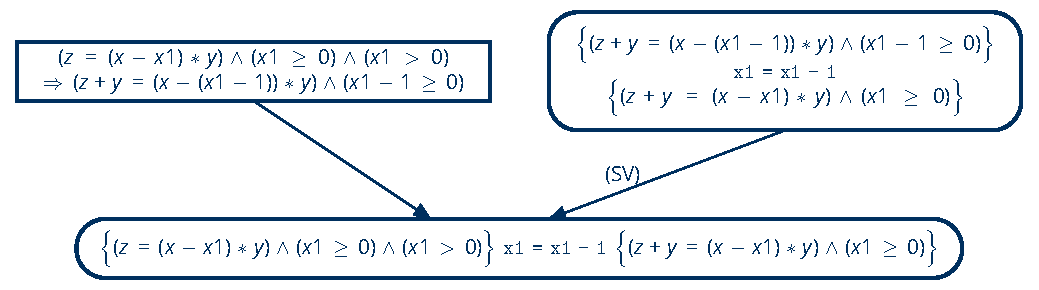
\includegraphics[width=\linewidth]{tut12-abb}
	\end{center}
	wobei (beachte: $x1$ ist Ganzzahl)
	\begin{align*}
		&(z = (x - x1) * y) \land (x1 \ge 0) \land (x1 > 0) \\
		\Rightarrow \enskip &(z + y = (x - x1) * y + y) \land (x1 \ge 0) \land (x1 > 0) \\
		\Rightarrow \enskip &(z + y = (x - x1 + 1) * y) \land (x1 \ge 0) \land (x1 > 0) \\
		\Rightarrow \enskip &(z + y = (x - (x1 - 1)) * y) \land (x1 \ge 0) \land (x1 > 0) \\
		\Rightarrow \enskip &(z + y = (x - (x1 - 1)) * y) \land (x1 \ge 0) \land (x1 - 1 \ge 0)
	\end{align*}
\end{frame}

\section{Aufgabe 3}

\begin{frame} \frametitle{Aufgabe 3 -- Teil (a)}
	\begin{figure}
		\centering
		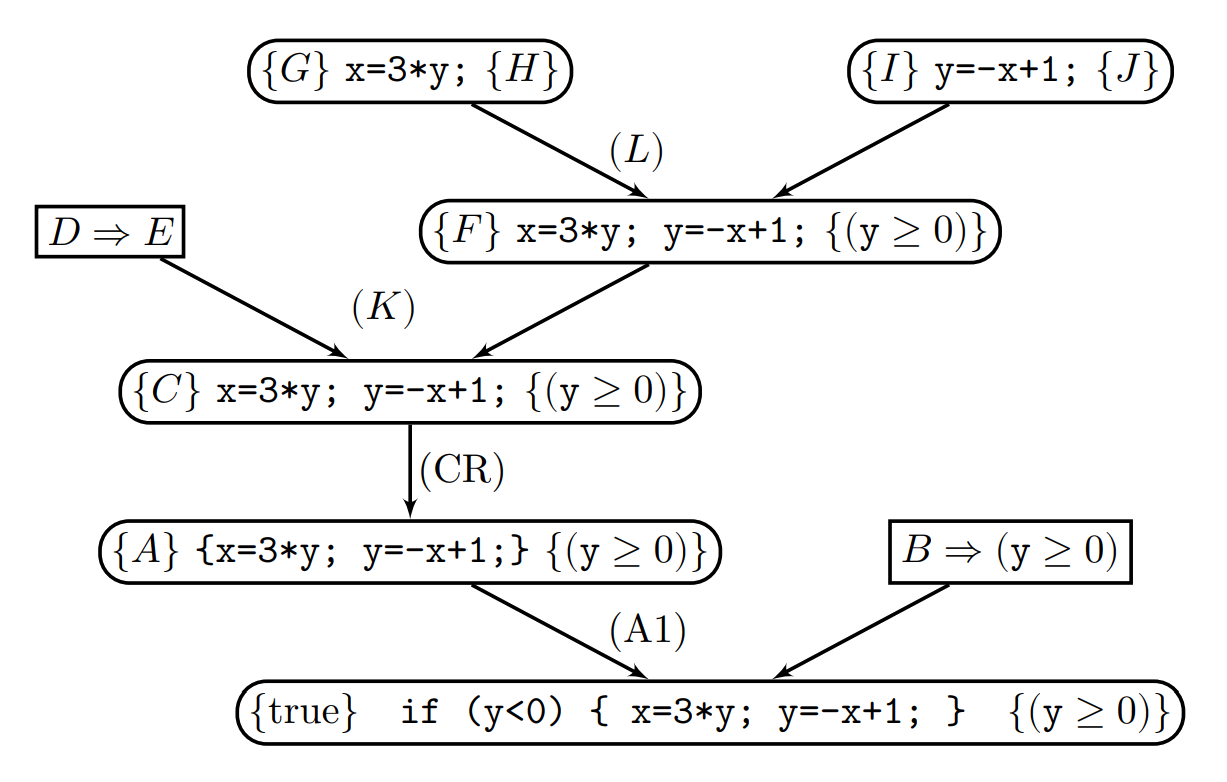
\includegraphics[width=\linewidth]{tut12-aufgabe3-baum.png}
	\end{figure}
\end{frame}

\begin{frame} \frametitle{Aufgabe 3 -- Teil (a)}
	\begin{minipage}{\dimexpr0.5\linewidth-\fboxrule-\fboxsep}
		\begin{align*}
			A &= \text{true} \logand (y < 0) \\
			B &= \text{true} \logand \lnot \ (y < 0) \\
			C &= A \\
			D &= A \\
			E &= ( -(3*y) + 1 \ge 0) \\
			F &= E 
		\end{align*}
	\end{minipage}
	\begin{minipage}{\dimexpr0.5\linewidth-\fboxrule-\fboxsep}
		\begin{align*}
		G &= E \\
		H &= (-x + 1 \ge 0) \\
		I &= H \\
		J &= (y \ge 0) \\
		K &= \text{stärkere Vorbedingung} \\
		L &= \text{Sequenzregel} 
		\end{align*}
	\end{minipage}	
\end{frame}

\begin{frame}[t] \frametitle{Aufgabe 3 -- Teil (b)}
	\begin{center}
		\textbf{zu zeigen:} $\text{true} \ \land \ (y < 0) \enskip \Rightarrow \enskip (-3 * y + 1 \ge 0)$
		\pause
		\begin{alignat*}{2}
			\text{true} \ \land \ (y < 0) \enskip &\Rightarrow \quad &y &< 0 \\
			&\Rightarrow \quad &-3 * y &> 0 \\ 
			&\Rightarrow \quad &-3 * y + 1 &> 1 \\ 
			&\Rightarrow \quad &-3 * y + 1 &\ge 0 
		\end{alignat*}
	\end{center}
\end{frame}

\end{document}

